
% - Description du capteur
% 		- Le matériel
% 		- Le système d'exploitation Zephyr
% 		- La couche radio LoRa
%      - Le logiciel embarqué
%		- Le boîtier

\chapter{Description du capteur}\label{ch:capteur}

Le travail du capteur et d'acquérir les données nécessaires, puis de les transmettre à intervalles réguliers par la couche radio LoRa aux passerelles. Le cœur du capteur est le micro-contrôleur, celui-ci permet l'exécution du firmware qui est en charge de la gestion des opérations. C'est cette application qui va effectuer aux moments voulus les acquisitions nécessaire et ensuite créer un paquet de données pour être  envoyé.

Pour se faire le capteur est munit de plusieurs modules permettant l'acquisition des différents paramètres. Il sont présentés dans la liste suivante.

\begin{itemize}
\item GPS: Il permettra de connaître la position (latitude/longitude) du capteur et également d'avoir une référence de temps
\item Accéléromètre: Ce module sera utilisé pour connaître le nombre de pas effectués par le sportif ce qui permettra de calculer sa cadence de course
\item Rythme cardiaque:  Au moyen d'une sangle pectorale portée par l'athlète, ce module déclenchera une impulsion à chaque fois qu'un battement du cœur sera détecté
\item Radio LoRa: C'est au moyen de cet élément que le capteur transmettra les paquets de données à la passerelle
\end{itemize}

\section{Le matériel}

Lors de la pré-étude du projet, trois différentes cartes avaient été étudiée chacune avec leurs avantages et inconvénients. Pour la réalisation du projet, j'ai décidé d'utiliser la carte qui dispose de base du plus de module, c'est à dire la carte SODAQ One. En effet elle a l'immense avantage d'embarquer de base un module LoRa, un module GPS ainsi qu'un accéléromètre ce qui me permet de me focaliser sur le développement du logiciel embarqué. Il reste seulement à connecter sur une entrée du micro-contrôleur le module qui permettra de compter les battements du cœur en détectant les impulsions produite. Enfin afin de faciliter le debug de l'application embarquée, un UART et une sonde de debug seront également connectés pendant la phase de debug ce qui permettra d'afficher des messages et de permettre le debug du firmware. Un autre avantage de taille est que son micro-contrôleur est déjà disponible dans le système d'exploitation Zephyr ce qui facilitera le travail de portage.

Pour rappel, les caractéristiques du SODAQ One sont décrit dans la table~\ref{tab:sodaq_one_cara}.

\begin{table}[htb]
\caption[Caractéristiques de la carte SODAQ One v3]{Caractéristiques de la carte SODAQ One v3}
\label{tab:sodaq_one_cara}
\centering
\begin{tabular}{ l | l }
\toprule
Dimensions & 45mm x 25mm \\
\midrule
Microcontrôleur & ATSAMD21G18 – ARM Cortex M0 \\
\midrule
Oscillateur & 48 Mhz \\
\midrule
Flash & 256 kB \\
\midrule
RAM & 32 kB \\
\midrule
LoRa & Microchip RN2483 \\
\midrule
GPS & uBlox EVA 8M \\
\midrule
Accéléromètre & STMicroelectronics LSM303AGR \\
\midrule
Prix & 114 CHF\\
\bottomrule 
\end{tabular}
\end{table}

Aux modules de base, comme expliqué précédemment, il faudra rajouter un module qui permettra de compter le nombre de battement du cœur. Il est développé par la société Adafruit sous le nom de "Adafruit Heart Rate Start Pack".

\hl{PHOTO SODAQ}

Le module LoRa RN2483 est connecté par un lien série UART et utilise une interface de type AT commands, c'est à dire qu'il est piloté avec l'envoie de chaînes de caractère représentant des commandes, dans la même idée les réponses reçues sont de type text. Le module GPS ainsi que l'accéléromètre sont quant à eux connecté sur le bus $I^{2}C$. Le module rythme cardiaque sera lui connecté simplement sur un General Purpose I/O.

% Configuration HW? i.e. nb msg GPS etc..

Le schéma block~\ref{fig:schema_block_sodaq} présente les différents modules et leurs connections avec le micro-contrôleur.

\hl{Ajouter debug SEGGER}

\begin{figure}[htb]
\centering 
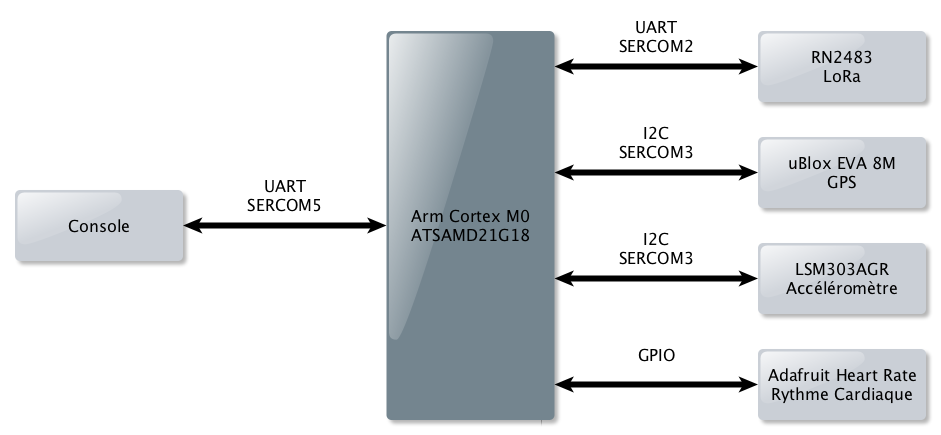
\includegraphics[width=1\columnwidth]{sensor_schema} 
\caption{Schéma block du capteur SODAQ One}
\label{fig:schema_block_sodaq}
\end{figure}

\section{Le système d'exploitation Zephyr}

Zephyr project ou Zephyr est un système d'exploitation temps réel (RTOS) open source réalisé par la Linux Foundation. Il a été développé pour être utilisé sur des petits systèmes embarqués avec de grosses contraintes au niveau des ressources à disposition. A sa base il reprend un "micro" noyau développé par la société Wind River pour son système d'exploitation commercial VxWorks qui est employé dans beaucoup de projet dans les domaines aérospatial, militaire et automobile.
Plusieurs architectures de micro-contrôleur sont pris en charge comme ARM, RISC ou x86 par exemple et plusieurs dizaines de configuration pour différentes cartes du marché existent. 

Ce RTOS est également très facile a configurer pour ses propres besoins au moyen de fichiers de configuration ou l'on peut sélectionner les éléments que l'on veut utiliser dans son application. De plus il propose toutes les fonctionnalités que l'on peut attendre de ce genre de système: scheduler, thread, semaphore, message queue, ring buffer, gestion de l'allocation de la mémoire dynamiquement...
En plus de ces fonctions de base il dispose également de drivers pour piloter différents types de composants comme des UART, SPI, ADC ou GPIO par exemple. Enfin des couches réseaux tel que Ethernet, IPv6 ou Bluetooth sont disponible ainsi que la gestion de système de fichier. \cite{zephyr_web}

Autour de cet RTOS Il existe une importante communauté qui travail activement sur son développement ce qui permet de pouvoir avoir des réponses à ses questions rapidement et efficacement.

Ce système d'exploitation a été choisi car en plus d'être moderne il dispose déjà de la configuration d'une carte très similaire au SODAQ One, le Adafruit Feather M0 Basic Proto qui embarque le même micro-contrôleur, ceci facilitera passablement le travail de modifications pour adapter la configuration du RTOS au SODAQ One. Cette configuration consiste a définir, grâce à des Device Tree, quels sont les composants que la carte embarque et sur quels ports ou pins ils sont connectés, cela permet ensuite au système d'exploitation de pouvoir les piloter correctement.

Même si beaucoup d'éléments sont déjà existant pour le micro-contrôleur utilisé par le SODAQ One, le développement d'un drivers $I^{2}C$ a été réalisé car il n'en n'existait aucun au moment ou j'ai commencé le travail de Bachelor. Ce driver est utilisé afin de pouvoir communiquer avec les modules GPS et accéléromètre. Les drivers développé dans le cadre du travail de diplôme sont décrit en détail dans la section \ref{ch:drivers}.

La figure \ref{fig:zephyr_archi} présente l'architecture système du système d'exploitation temps-réel Zephyr.

\begin{figure}[htb]
\centering 
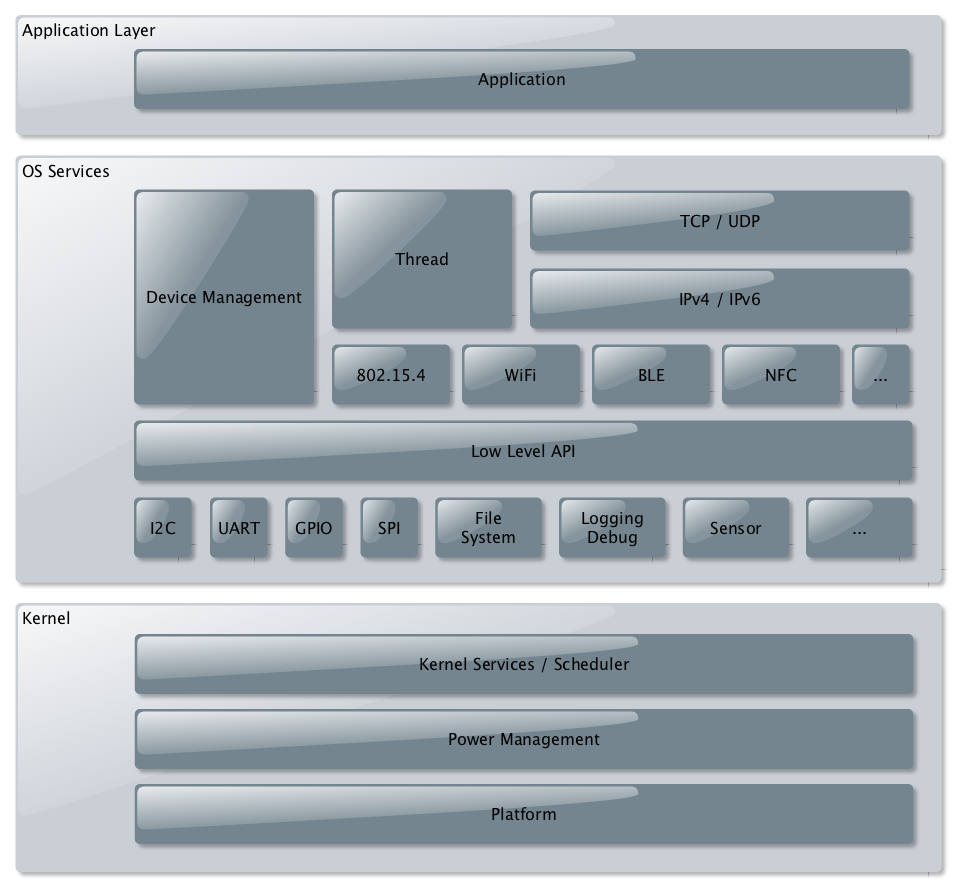
\includegraphics[width=0.8\columnwidth]{zephyr_archi} 
\caption{Architecture système du système d'exploitation Zephyr - http://www.zephyrproject.org}
\label{fig:zephyr_archi}
\end{figure}

\section{Les drivers}\label{ch:drivers}

Afin de pouvoir utiliser tous les modules requis par le projet ainsi que le RTOS Zephyr il a été nécessaire d'écrire plusieurs drivers qui sont décrits dans cette section.

Les drivers présenté dans la liste suivante ont été développés dans le cadre du travail de Bachelor.

\begin{itemize}
\item Driver $I^{2}C$ pour micro-contrôleur ATSAMD21G18 intégré au système d'exploitation Zephyr
\item Driver UBloxEVA8M pour piloter le module GPS qui se base lui même sur le driver $I^{2}C$
\item Driver LSM303AGR pour le module accéléromètre qui se base également sur le driver  $I^{2}C$
\item Driver RN2483 LoRa permettant d'exploiter la communication LoRa et qui se base sur le driver UART existant de Zephyr
\item Driver pour piloter les 3 LEDs de la carte SODAQ One au travers de GPIOs
\end{itemize}

\subsection{Driver $I^{2}C$ ATSAMD21G18}

\hl{TODO Ajouter data sheet SAMD21 dans biblio + réf}

$I^{2}C$ est un bus qui permet de connecter plusieurs esclaves à un maître. Le maître est le seul à initier les accès aux esclaves qui disposent chacun de leur adresse spécifique, lorsque le maître veut lire ou écrire sur un esclave il va envoyer un message $I^{2}C$ contenant l'adresse de l'esclave en question, suivi des données à écrire ou de l'adresse à lire par exemple. Avantage de taille est qu'il ne nécessite que deux connections pour fonctionner, une qui permet la distribution du signal de synchronisation qui est uniquement contrôlé par le maître et une autre pour le transfert des données qui peut être contrôlé soit par le maître lors d'une écriture ou de l'esclave pour une lecture.

\begin{figure}[htb]
\centering 
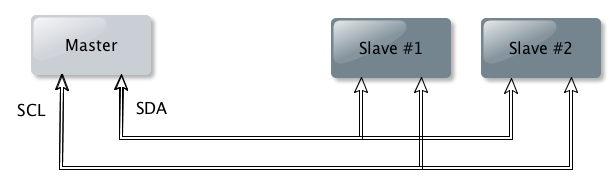
\includegraphics[width=0.8\columnwidth]{i2c_bus} 
\caption{Schéma d'un bus $I^{2}C$}
\label{fig:i2c_bus}
\end{figure}

Le bus $I^{2}C$ utilise un protocole pour la communication entre un maître et un esclave, en fonction de l'opération voulue le message ne sera pas tout à fait le même. Le maître commence toujours par envoyer l'adresse de l'esclave à qui est destiné le message, suivi de l'opération, lecture ou écriture. Les données sont ensuite placé sur le bus par le maître dans le cas d'une écriture ou par l'esclave lors d'une lecture. Chose importante lorsque le maître à terminé le processus de lecture, il doit envoyé un message de type NACK suivi d'un STOP afin d'informer l'esclave de la fin du transfert.
La figure \ref{fig:i2c_messages} propose les deux types de messages qu'il existe.

\begin{figure}[htb]
\centering 
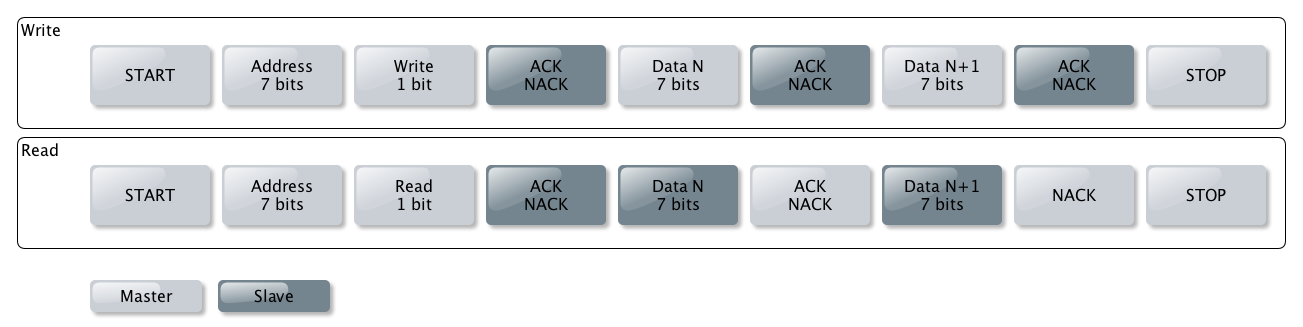
\includegraphics[width=1\columnwidth]{i2c_messages} 
\caption{Les messages $I^{2}C$}
\label{fig:i2c_messages}
\end{figure}

Le driver $I^{2}C$ est responsable du pilotage d'un des 5 SERCOM que propose le micro-contrôleur, ce sont des modules qui peuvent être configuré afin de proposer une interface de type UART, $I^{2}C$ ou SPI. Étant donné qu'il est intégré directement à Zephyr, il doit respecter les contraintes qui y sont liées c'est à dire d'être placé dans le dossier $I^{2}C$ du système d'exploitation: zephyr/drivers/i2c/i2c\_sam0.c et qu'il doit proposer une interface standardisée qui permet au système d'exploitation d'initier les opérations suivantes.

\begin{itemize}
\item Configuration de l'interface
\item Transfert de donnée (Lecture/Écriture)
\end{itemize}

Pour se faire, il faut remplir une structure avec des pointeurs de fonctions qui sont ensuite appelés par le système d'exploitation au besoin. En plus de cela, il faut définir et configurer un device, c'est la structure utilisée par Zephyr qui sera ensuite utilisée par les applications afin de pouvoir communiquer sur le bus $I^{2}C$.

C'est le driver qui en fonction de l'opération à effectuer va envoyer les codes (START ou STOP) suivie des données. Il produira les acquittement nécessaire et Il vérifiera également que l'esclave en question valide bien les messages. L'utilisation d'une l'interruption permet au driver de savoir, après avoir écrit un message dans le SERCOM, quand il a été effectivement envoyé ceci afin de pouvoir initier l'envoie du prochain message.

La figure \ref{fig:driver_i2c_uml} présente le diagramme de classe du driver $I^{2}C$.

\begin{figure}[htb]
\centering 
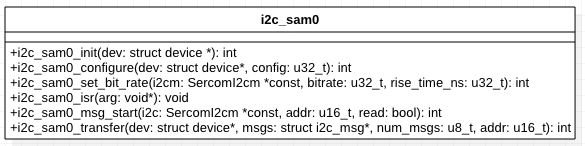
\includegraphics[width=0.8\columnwidth]{driver_i2c_uml} 
\caption{Diagramme de class du driver $I^{2}C$}
\label{fig:driver_i2c_uml}
\end{figure}

\subsection{Driver UBloxEVA8M}

Le driver UBloxEVA8M permet le pilotage du module GPS du même nom qui se trouve connecté sur le bus $I^{2}C$. Ce module est intégré directement à la carte SODAQ One et propose une gestion GPS complète, il est capable de recevoir les signaux GPS, GLONASS, QZSS et SBAS, il est extrêmement sensible, très rapide et de petite taille, en somme une solution idéal pour des capteurs de petite taille. Il est décrit en plus détails au chapitre \ref{ubloxeva8m_description}. 
\hl{TODO Chapitre GPS module link}

Le module utilise trois types de protocole pour la transmission des données et la configuration du module, NMEA, UPX et RTCM. NMEA est un protocole à base de texte qui envoie des messages formée de character ASCII il est idéale lorsque le module est connecté sur un UART. UPX est un protocole compact car il utilise des mots binaires qui sont protégés par des checksum. Enfin le protocole Radio Technical Commission for Maritime Services (RTCM) est unidirectionnel (seulement envoie vers le receveur) qui permet au receveur l'utilisation des corrections du positionnement relatif uniquement.
Le driver utilise uniquement le protocole UPX car il est le mieux adapté pour l'utilisation sur un bus $I^{2}C$, il est décrit en détail dans le document \cite{ublox-protocol}.

Une fois que le module a été configuré, il va produire les messages qui ont été activés et contenant diverses informations et les placé dans une FIFO. Au travers du bus $I^{2}C$, le thread du driver va interroger le module périodiquement afin de savoir si des messages sont prêt à être lu, si c'est le cas le driver va lire les messages disponible et les stocker dans une structure de type ubloxeva8m\_ubx\_msg. L'utilisateur récupère les messages reçu grâce à une fonction callback qui est passée au driver et qu'il appelle à chaque fois qu'un message est prêt.

Dans le cadre du projet, un seul message est utilisée c'est le UBX-NAV-PVT, la liste suivante présente un résumé des informations contenue dans ce mesage, pour plus de détails voir \cite[p.~307]{ublox-protocol}.

\begin{itemize}
 \item La date du jour
 \item L'heure actuelle 
 \item Le type de fix GPS
 \item La validité et la précision des informations contenus dans le message
 \item La latitude et longitude
 \item Le nombre de satellite actuellement vu
 \item La vitesse
 \end{itemize} 

\hl{TODO}

En ce basant sur le driver $I^{2}C$ décrit à la section précédente il va permettre l'initialisation, la configuration et la récupération des messages GPS du composant. Il utilise un thread qui va périodiquement 

La figure \ref{fig:driver_ubloxeva8m_uml} présente le diagramme de classe du driver UBloxEVA8M.

\begin{figure}[htb]
\centering 
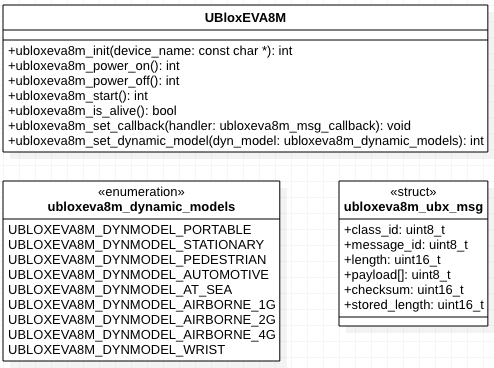
\includegraphics[width=0.8\columnwidth]{driver_ubloxeva8m_uml} 
\caption{Diagramme de class du driver UBloxEVA8M}
\label{fig:driver_ubloxeva8m_uml}
\end{figure}







\subsection{Driver LSM303AGR}

\subsection{Driver RN2483}

\subsection{Driver LEDs}


\section{Le logiciel embarqué}

\hl{TODO}

\section{Le boîtier}

\hl{TODO}
